\documentclass[10pt,a4paper,notitlepage]{article}
\usepackage[utf8]{inputenc}
\usepackage{amsmath}
\usepackage{amsfonts}
\usepackage{amssymb}
\usepackage{fullpage}
\usepackage{lastpage}
\usepackage{lscape}
\usepackage{fancyhdr}
\usepackage{multirow}
\usepackage{fancyvrb}
\usepackage{xcolor}
\usepackage{tikz}
\usepackage{graphicx}
\graphicspath{{./Graphics/}}
\usepackage{float}
\usepackage{nameref}
\usepackage[backend=bibtex,style=authortitle-ibid]{biblatex}
\addbibresource{References.bib}
  
\author{Jonah Gibbon}

\pagestyle{fancy}
\fancyhf{}
\renewcommand{\headrulewidth}{0pt}
\cfoot{Page \thepage\ of \pageref{LastPage}}

\newcommand{\abs}[1]{\lvert#1\rvert}
\newcommand{\Z}{\mathbb{Z}}
\newcommand{\Q}{\mathbb{Q}}
\newcommand{\C}{\mathbb{C}}
\newcommand{\N}{\mathbb{N}}
\newcommand{\R}{\mathbb{R}}
\newcommand{\f}{\mathcal{F}}
\newcommand{\g}{\mathbf{g}}
\newcommand{\x}{\mathbf{x}}
\newcommand{\y}{\mathbf{y}}
\newcommand{\s}{\mathbf{s}}
\newcommand{\p}{\mathbf{p}}
\newcommand{\q}{\mathbf{q}}
\newcommand{\h}{\mathbf{H}}
\newcommand{\A}{\mathbf{a}}
\newcommand{\B}{\mathbf{b}}
\newcommand{\G}{\mathbf{G}}
\newcommand{\X}{\mathbf{X}}
\newcommand{\M}{\mathbf{M}}

\renewcommand{\theequation}{\textbf{\arabic{equation}}}
\renewcommand{\refname}{Reference}

\begin{document}
For the sake of this project, let $f$ denote the function in question, with it's minimum at $\x^{*}$. Equations referenced throughout the project will appear in \textbf{bold}, whereas equations referenced from the project booklet will appear as normal. \\

Throughout the project, the subroutine \texttt{lambda(x,s,d)} was used to calculate the value of $\lambda^{*}$ correct to $d+1$ significant figures given point $\x$ and direction $\s$. The codes do have the option to manually input the values of $\lambda^{*}$, however this is not effective when wanting to calculate $\lambda^{*}$ to a high accuracy. This subroutine is preferred over 'eyeballing' the value of $\lambda^{*}$ from graphs of $\phi(\lambda)$, and it will be stated explicitly which option is being used where. The subroutine is referenced on page \pageref{cd:0}.

\subsection*{\centering Question 1}
Below are the two contour plots of functions (4) and (5), produced by '\nameref{cd:0.5}', referenced on page \pageref{cd:0.5}. 
\begin{figure}[H]
\centering
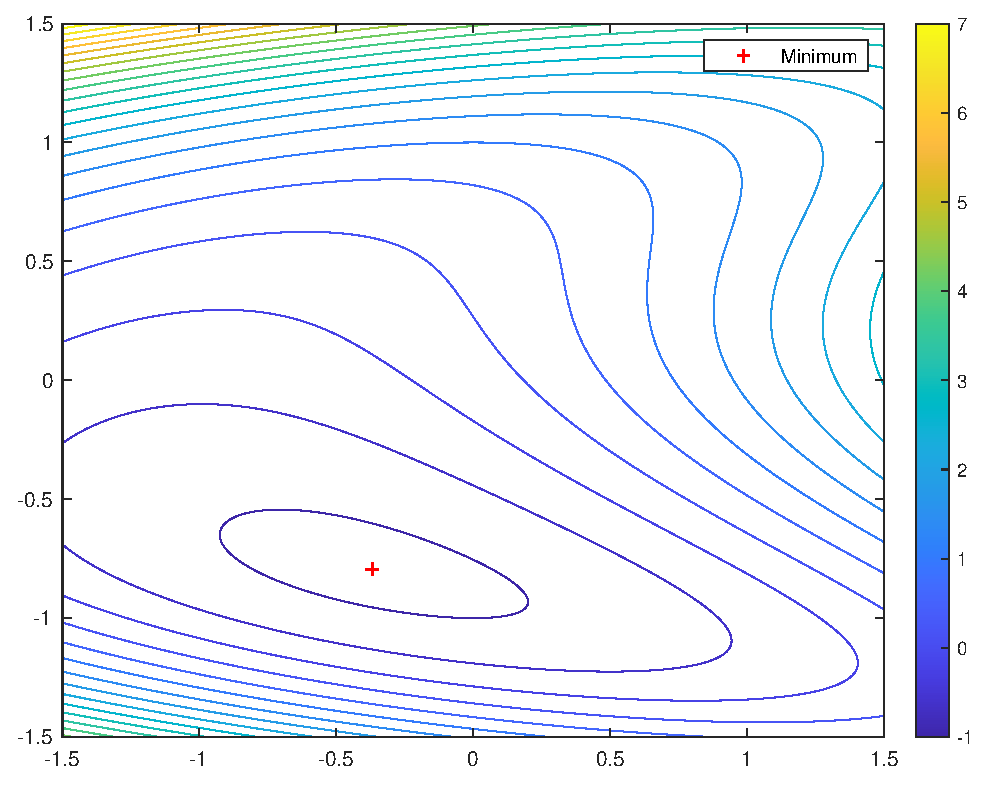
\includegraphics[width=9.5cm]{Image_1}
\caption{Contour plot of function (4)}\label{fg:1}
\end{figure}
\begin{figure}[H]
\centering
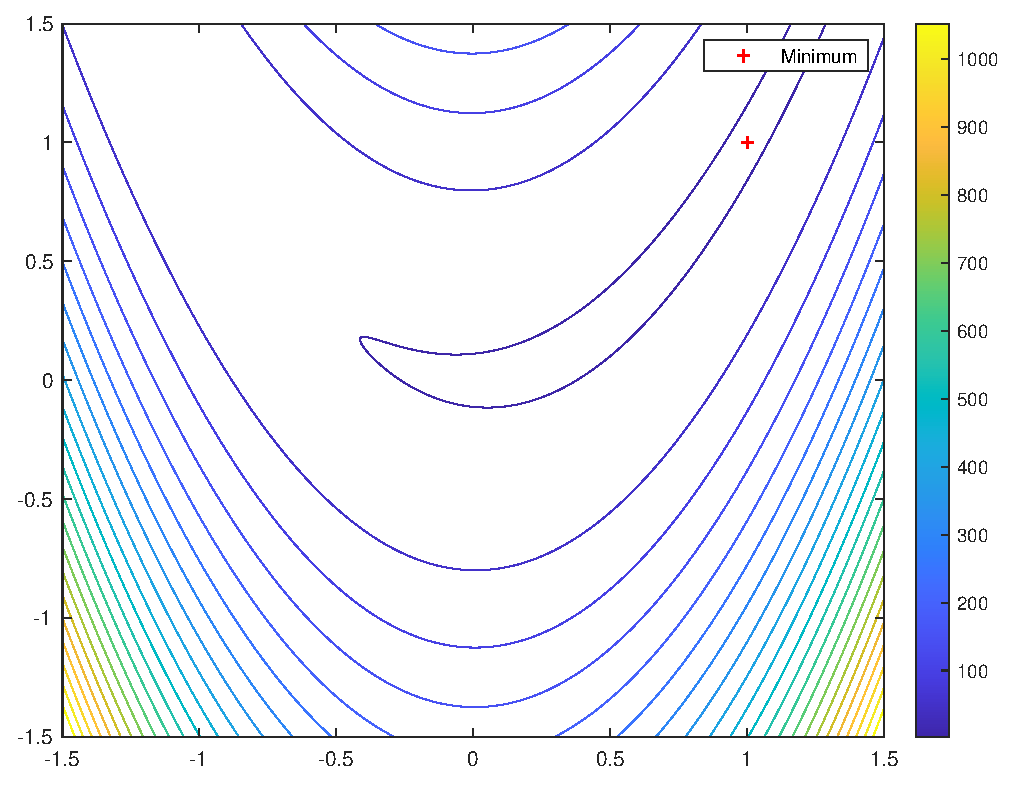
\includegraphics[width=9.5cm]{Image_2}
\caption{Contour plot of function (5)}\label{fg:2}
\end{figure}
The first minimum can be found by setting $\nabla f=0$, which yields two simulations equations. Solving these gives the solution $(2^{-2/3}-1,-2^{-1/3})$, with minimum value $-1/2-3/(4\sqrt[3]{2})$. This is indeed a minimum since the function is continuous, it uniquely solves $\nabla f=0$, and the function diverges to $+\infty$ as $\abs{\abs{\x}}$ tends to $\infty$. 

The minimum of equation (5) can be found immediately from minimising both terms, with solution at $(1,1)$ with $f(\x^{*})=0$. Both minima have been plotted on the above figures using a red cross. Notice that the contours of Figure \ref{fg:2} follow a parabolic shape, which is because it's second term is far more dominant than the first, and causes very steep sides when deviated from.
\subsection*{\centering Question 2}
All results in Questions 2-3 were produced by '\nameref{cd:1}', referenced on page \pageref{cd:1}, including being used to approximate the minimum of equation (4) using the steepest decent method. The numerical values of these iterates are included in Table \ref{tb:1}, and plotted graphically in Figure \ref{fg:3}. Note the difference of successive iterates $D_{i}=f(\x_{i})-f(\x_{i-1})$, and the ratio of differences were tabulated as well. The value of $d$ in the subroutine \texttt{lambda} was set to 5 (calculates $\lambda^{*}$ to $d+1=6$ significant figures).

\begin{table}[H]
\centering
\begin{tabular}{|cccccccc|} \hline $i$ & $x_{i}$ & $y_{i}$ & $\lambda^{*}$ & $f(\x_{i})$ & $\abs{\abs{\nabla f(\x_{i})}}$& $D_{i}$ & $D_{i}/D_{i-1}$ \\
\hline
0 & -1.0 & -1.3 & 0.082899 & 1.0561 & 7.969256 & $\ast$ & $\ast$ \\ 
1 & -0.8599007 & -0.6543826 & 1.65198 & -1.02119209 & 0.2948156 & -2.077292 & $\ast$ \\ 
2 & -0.3839367 & -0.7576102 & 0.157194 & -1.09200179 & 0.1985912 & -0.07080970 & 0.03408750 \\ 
3 & -0.3905530 & -0.7881184 & 1.72041 & -1.09514853 & 0.01195546 & -3.146733e-3 & 0.04443929 \\ 
4 & -0.3704524 & -0.7924796 & 0.149098 & -1.09527142 & 7.185838e-3 & -1.228923e-4 & 0.03905394 \\ 
5 & -0.3706796 & -0.7935267 & 1.72315 & -1.09527537 & 3.726467e-4 & -3.851406e-6 & 0.03133968 \\ 
6 & -0.3700521 & -0.7936629 & 0.148832 & -1.09527539 & 2.220084e-4 & -1.196418e-7 & 0.03106443 \\ 
7 & -0.3700591 & -0.7936952 & 1.7236 & -1.09527539 & 1.142352e-5 & -3.667890e-9 & 0.03065727 \\ 
8 & -0.3700399 & -0.7936994 & 0.148822 & -1.09527539 & 6.783482e-6 & -1.124629e-10 & 0.03066148 \\ 
9 & -0.3700401 & -0.7937004 & 1.72374 & -1.09527539 & 3.478657e-7 & -3.423928e-12 & 0.03044495 \\ 
10 & -0.3700395 & -0.7937005 & $\ast$ & -1.09527539 & 2.063366e-7 & -1.043610e-13 & 0.03047990 \\ \hline \end{tabular}
\caption{Iterates of Gradient Decent for equation (4)}\label{tb:1}
\end{table}
\begin{figure}[H]
\centering
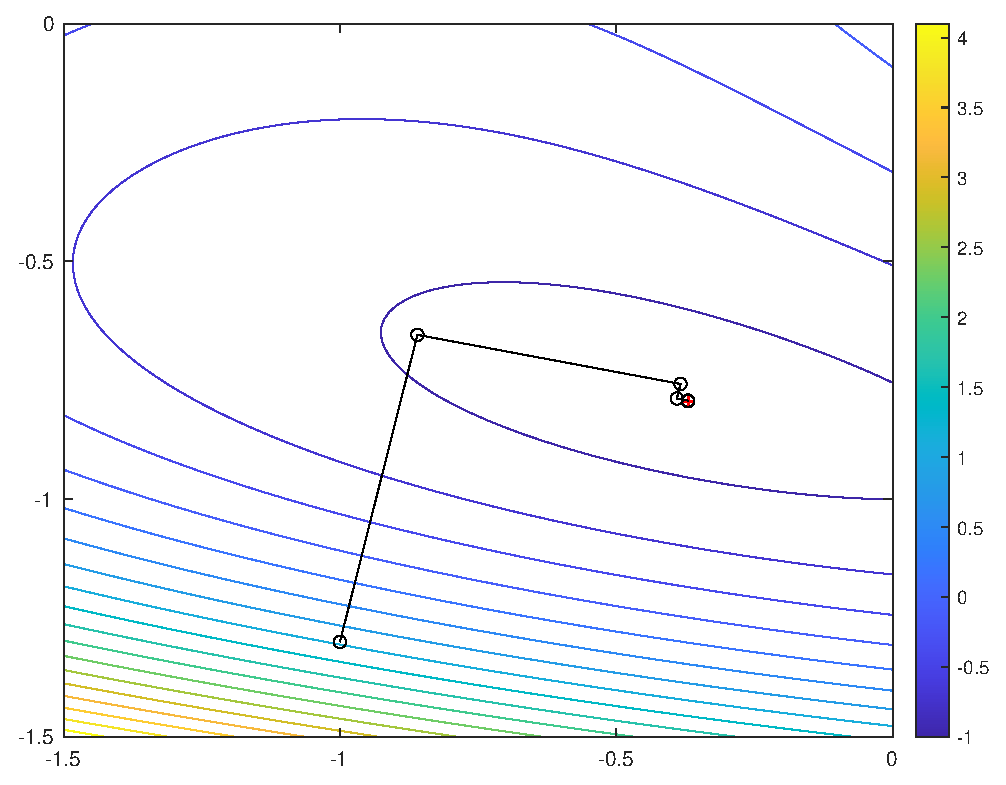
\includegraphics[width=11cm]{Image_3}
\caption{Graphical plot of data in Table \ref{tb:1}}\label{fg:3}
\end{figure}
First notice that the values in Table \ref{tb:1} have been rounded such that they fit in this document, each value was stored to 16 significant figures in the algorithm; the precision MATLAB uses. The final value of $f(\x_{10})=-1.09527539448807$.\par
Secondly notice that consecutive line segments of each iterate seem to be to orthogonal to one another. This is true in general, since if $\x_{n+1}=\x_{n}-\lambda_{n}^{*}\nabla f(\x_{n})$, and $\x_{n+2}=\x_{n+1}-\lambda_{n+1}^{*}\nabla f(\x_{n+1})$, then 
\begin{equation}
\left(x_{n+2}-x_{n+1}\right)^{T}\left(\x_{n+1}-\x_{n}\right)=\lambda_{n+1}^{*}\lambda_{n}^{*}\nabla f(\x_{n+1})^{T}\cdot\nabla f(\x_{n})
\end{equation}
But $\lambda_{n}^{*}$ was chosen to minimise $\phi_{n}(\lambda)=f(\x_{n}-\lambda \nabla f(\x_{n}))$, i.e 
\begin{equation}
\begin{aligned}
0 &= \frac{d\phi_{n}}{d\lambda}\left(\lambda_{n}^{*}\right)\\
&= -\nabla f(\x_{n})^{T}\cdot \nabla f\left(\x_{n}-\lambda_{n}^{*}\nabla f(\x_{n})\right)\\
&= -\nabla f(\x_{n})^{T}\cdot \nabla f(\x_{n+1})
\end{aligned}
\end{equation}
hence they are orthogonal.\\

Aside: Throughout this project, the ratio of differences $D_{i}$ and $N$-step differences $A_{i}=f(\x_{(i+1)N})-f(\x_{iN})$ will be investigated to (roughly) determine the order of convergence of said method. Should $D_{i}/(D_{i-1})^{p}$ be constant asymptotically, we claim that this method is a $p$-th order convergent method. A simple proof of this can be found in \cite{111}.\\

We can see the ratio of differences between iterates in Table \ref{tb:1} (represented in column 7) has roughly constant value $\mu =0.0305$. Assuming this is true for all following iterates, we may extrapolate to find a better value of $f(\x^{*})$
\begin{equation}
\begin{aligned}
f(\mathbf{x}_{*})&= \lim_{n\rightarrow \infty} \left( f(\mathbf{x}_{n})-f(\mathbf{x}_{n-1})+f(\mathbf{x}_{n-1})-\hdots -f(\mathbf{x}_{9})\right) +f(\mathbf{x}_{9})\\
&\approx \lim_{n\rightarrow \infty} D_{10}\left(1 + \mu + \hdots + \mu^{n}\right)+f(\mathbf{x}_{9})\\
&=f(\mathbf{x}_{9})+\frac{D_{10}}{1-\mu}=-1.09527539448817
\end{aligned}
\end{equation}
The fact that $D_{i}/D_{i-1}$ is roughly constant implies that this method is converging linearly to the exact solution.\\

The successive values of $\abs{\abs{\x_{n}-\x_{n-1}}}$ were also calculated, along with their ratios. The data is plotted below in Table \ref{tb:9}.
\begin{table}[H]
\centering
\begin{tabular}{|ccc|} \hline $n$ & $R_{n}=\abs{\abs{\x_{n}-\x_{n-1}}}$ & $R_{n}/R_{n-2}$\\
\hline 1 & 0.660643 & $\ast$\\ 
2 & 0.487029 & $\ast$ \\ 
3 & 0.0312173 & 0.0472529\\ 
4 & 0.0205683 & 0.0422321\\ 
5 & 1.07139e-3 & 0.0343205\\ 
6 & 6.42126e-4 & 0.0312192\\ 
7 & 3.30420e-5 & 0.0308402\\ 
8 & 1.96896e-5 & 0.0306631\\ 
9 & 1.00953e-6 & 0.0305530\\ 
10 & 5.99630e-7 & 0.0304542\\ \hline 
\end{tabular}
\caption{Investigation of $R_{n}=\abs{\abs{\x_{n}-\x_{n-1}}}$}\label{tb:9}
\end{table}
By calculating $R_{n}/R_{n-2}$, we can see how the distance between consecutive parallel iterates behave. The data suggests that they also converge linearly, with approximately the same value $\mu=0.031$. Using the same method as above, it suggests that $\x^{*}$ will lie in a rectangular region with semi major axis $\max\left(R_{9},R_{10}\right)/1-\mu$ and semi minor axis $\min\left(R_{9},R_{10}\right)/1-\mu$, centred at $\x_{10}$.  This rectangle will be rotated such that the axis are parallel with the iterates. Using the data in Table \ref{tb:9}, we estimate that $\x^{*}$ lies in said rectangle with major/minor axis $(1.0413\times 10^{-6},6.1849\times 10^{-7})$. centred at $\x_{10}$ and rotated such that the major axis is parallel with $\nabla f(\x_{0})$.\\

Suppose the function near the minimum $\x^{*}$ was strongly convex with parameter $m>0$, i.e.
\begin{equation}\label{eq:SC}
f(\mathbf{y})\geq f(\mathbf{x}) +\nabla f(\x)^{T}\left(\y-\x\right)+\frac{m}{2}\abs{\abs{\y-\x}}^{2}
\end{equation}
for all $\x,\y$ in some neighbourhood around $\x^{*}$. By taking derivatives of the RHS with respect to $\y$, we find $\widetilde{\y}=\x-(1/m)\nabla f(\x)$ minimises the RHS. We therefore deduce the lower bound
\begin{equation}
\begin{aligned}
f(\y) &\geq f(\x) +\nabla f(\x)^{T}\left(\widetilde{\y}-\x\right) + \frac{m}{2}\abs{\abs{\widetilde{\y}-\x}}^{2}\\
&= f(\x)-\frac{1}{2m}\abs{\abs{\nabla f(\x)}}^{2}
\end{aligned}
\end{equation}
Notice this lower bound stays true for all values of $\y$, so by setting $\y=\x^{*}$ and $\x=\x_{n}$ we deduce that
\begin{equation}\label{eq:4}
f(\x_{n})-f(\x^{*})\leq \frac{1}{2m}\abs{\abs{\nabla f(\x_{n})}}^{2}
\end{equation}
This allows us to ensure that our approximation to the minimum value is close to the real value, just by evaluating the gradient near the minimum. By setting $\x=\x^{*}$ and $\y=\x_{n}$ in equation \eqref{eq:SC}, and using the results from equation \eqref{eq:4}, we deduce
\begin{equation}\label{eq:7}
\abs{\abs{\x_{n}-\x^{*}}}\leq \sqrt{\frac{2}{m}}\sqrt{f(\x_{n})-f(\x^{*})}\leq\frac{1}{m}\abs{\abs{\nabla f(\x_{n})}}
\end{equation}
Therefore the optimal solution will lie in a circle of small radius around the most recent iterate. Using both these results, we can write effective termination statements in the code, dependant on how small $\abs{\abs{\nabla f(\x_{n})}}$ is.\\

We can analytically calculate $m$. Function (4) is strongly convex if and only if $h(\x)=f(\x)-m\abs{\abs{\x}}^{2}/2$ is convex. The Hessian of $h(\x)$ is equal to
\begin{equation}
H= \begin{pmatrix}
1-m & -2y \\
-2y & 12y^{2}-2(1+x)-m
\end{pmatrix}
\end{equation}
By taking determinants of upper left sub matrices (Sylvester's Criterion), we deduce this function is strongly convex if $m<1$ and $4(2-3m)y^{2}-2(1-m)x+(m+2)(m-1)>0$. This second condition describes the left side of a parabola in the Euclidean plane, in which the root must lie. Therefore we must choose
\begin{equation}
\begin{aligned}
m &<\frac{-2x+12y^{2}-1-\sqrt{\left(12y^{2}-2x-1\right)^{2}-4\left(8y^{2}-2x-2\right)}}{2}\\
&=\frac{5\times 2^{1/3}+1-\sqrt{25\times 2^{2/3}-2\times 2^{1/3}+1}}{2}\approx 0.561
\end{aligned}
\end{equation}
For any $m$ chosen to be less than this constant, there exists some neighbourhood around the root such that the function $f(\x)$ is strongly convex. Assuming $\x_{10}$ lies within this neighbourhood, we deduce from equation \eqref{eq:7} that the root \textit{definitely} lies within a circle centred at $\x_{10}$ with radius approximately $3.678\times 10^{-7}$. We can also deduce that $f(\x^{*})$ lies between $f(\x_{10})\pm 3.795\times 10^{-14}$. Notice this agrees with the extrapolated results above, however these better intervals were calculated by already knowing where the minimum was.

\subsection*{\centering Question 3}
The first 25 iterations of the algorithm for function (5),are plotted below in Figure \ref{fg:4}.
\begin{figure}[H]
\centering
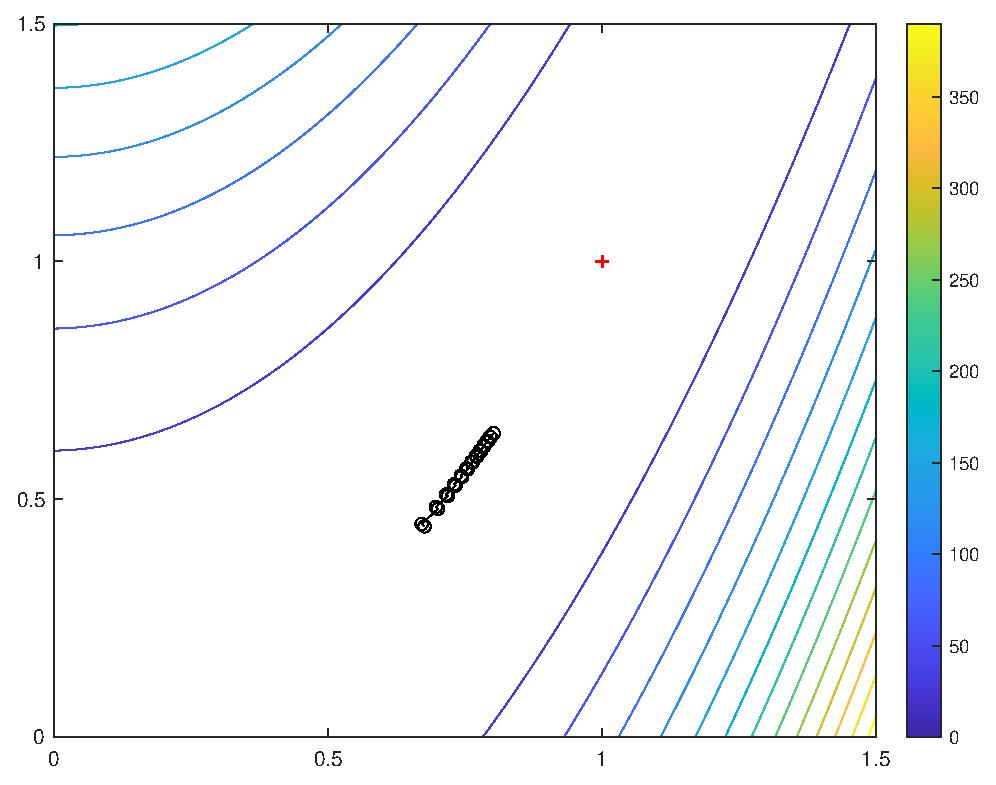
\includegraphics[width=11cm]{Image_4}
\caption{SD Algorithm for Function (5)}\label{fg:4}
\end{figure}
We can see that the iterations are moving towards the minimum very slowly. This is loosely due to the fact that successive iterations must be perpendicular to one another. This puts a tight bound on which directions the iterations can take, based on the initial starting point, since the sides of the valley the iterates converge along is incredibly steep. We will investigate the rate of convergence of these iterates throughout the rest of this question.
\subsubsection*{\centering Convergence of Steepest Decent Method}
Suppose there existed constants $m, M>0$ such that
\begin{equation}
\begin{aligned}
f(\y) &\geq f(\x) +\nabla f(\x)^{T}(\y-\x)+\frac{m}{2}\abs{\abs{\y-\x}}^{2}\\
f(\y) &\leq f(\x) +\nabla f(\x)^{T}(\y-\x)+\frac{M}{2}\abs{\abs{\y-\x}}^{2}
\end{aligned}
\end{equation}
for all $\x,\y$ in some region near $\x^{*}$. This is equivalent to $f$ satisfying the condition $mI\preceq f(\x)\preceq MI$. If we choose $\y=\x_{n+1}=\x_{n}-\lambda^{*}\nabla f(\x_{n})$ and $\x=\x_{n}$ then
\begin{equation}
\begin{aligned}
f(\x_{n+1})=f\left(\x_{n}-\lambda^{*}\nabla f(\x_{n})\right) &\leq f\left(\x_{n}-\frac{1}{M}\nabla f(\x_{n})\right)\\
&\leq f(\x_{n})-\frac{1}{M}\abs{\abs{\nabla f(\x_{n})}}^{2}+\frac{M}{2}\abs{\abs{\frac{1}{M}\nabla f(\x_{n})}}^{2}\\
&=f(\x_{n})-\frac{1}{2M}\abs{\abs{\nabla f(\x_{n})}}^{2}
\end{aligned}
\end{equation}
Using the results of equation \eqref{eq:4} we deduce that
\begin{equation}
f(\x_{n+1})-f(\x^{*})\leq \left(1-\frac{m}{M}\right)\left(f(\x_{n})-f(\x^{*})\right)
\end{equation}
We can see that this method will not just always converge, but at least as fast as linear convergence, with constant $\kappa=(1-m/M)$, as long as the iterates remain in the region where $f(x)$ is strongly convex.\footnote{The results above were inspired from the lectures \cite{Caramanis}.} We can prove that the coordinates $\x_{n}$ converge to $\x^{*}$ with linear convergence too, however it relies on the fact that this method is globally convergent.\footnote{This will be proved later in Question 5, since it is a direct result of the global convergence of the Conjugate Gradient Method, and so will be assumed true from now on.} If we can argue that $\lambda^{*}_{n}$ is a function of $\x_{n}$, then we may express $\x_{n+1}$ as
\begin{equation}
\x_{n+1}=\x_{n}-\lambda^{*}_{n}\nabla f(\x_{n})=\x_{n}-g(\x_{n})
\end{equation}
for some function $g(\x)$. Note that $\x^{*}$ is a fixed point of the above, and thus we transform the steepest descent method into a fixed point iteration in multiple variables. By Taylor expanding the above about $\x^{*}$, we deduce 
\begin{equation}
\x_{n+1}=\x^{*}+\M\left(\x_{n}-\x^{*}\right)+O(\abs{\abs{\x_{n}-\x^{*}}}^{2})
\end{equation}
where $\M$ depends on the derivatives of $g$. Thus asymptotically we deduce that
\begin{equation}
\frac{\abs{\abs{\x_{n+1}-\x^{*}}}}{\abs{\abs{\x_{n}-\x^{*}}}}\leq \abs{\abs{\M}}
\end{equation}
and hence the coordinates will converge to $\x^{*}$ at least as fast as linear convergence. Notice all these results proved are consistent with the data produced in Question 2 (it is trivial to see that from linear convergence the ratios in Question 2 must be constant).
\subsubsection*{\centering Strong convexity of function (5)}
To find approximate values for $\kappa$, we must first calculate $m$ and $M$ from functions (4) and (5). Applying the same method as earlier (the workings have been removed for the brevity of this question), we calculate
\begin{table}[H]
\centering 
\begin{tabular}{|c|ccc|}
\hline Function & $m$ & $M$ & $\kappa$\\
\hline
(4) & 0.561 & 6.74 & 0.9167\\
(5) & 0.399 & 801.6 & 0.9995\\
\hline
\end{tabular}
\caption{Strong convexity parameters for functions (4) and (5)}
\end{table}

Comparing values of $\kappa$ explains the far slower convergence of function (5). It's estimated that for every iteration of the steepest descent method on function (4), it takes $\ln(0.9167)/\ln(0.9995)=174$ iterations for function (5) to converge to the same accuracy.\\

The first 25 iterates of the algorithm were calculated using a range of accuracies of $\lambda^{*}$ (using the subroutine \texttt{lambda}). The number of significant figures it was calculated to ranged from 2 to 8, and the distance the 25th iterate was from the minimum (1,1) was calculated to give an indication of how well the algorithm did. This data is tabulated below in Table \ref{tb:2}.
\begin{table}[H]
\centering
\begin{tabular}{c|c}
$d$ & $\abs{\abs{\x_{25}-\x^{*}}}$\\
\hline 1 & 0.031188\\
2 & 0.099985\\
3 & 0.38759\\
4 & 0.40933\\
5 & 0.41125\\
6 & 0.41142\\
7 & 0.41144\\

\end{tabular}
\caption{$\abs{\abs{\x_{25}-\x^{*}}}$ for different accuracies of $\lambda^{*}$}\label{tb:2}
\end{table}
We can see that as the accuracy improves, the method converges slower. This is because as $\lambda$ becomes closer to its true value $\lambda^{*}$, the iterates become more orthogonal, and hence more restricted in how this method evolves. So when $\lambda$ is less accurate, it's more 'likely' that one of the directions $\s_{n}$ points closer to the minimum, and hence can take one large step towards it. Finally notice that as the accuracy increases, the paths become more and more similar, and hence the point $\x_{25}$ begins to look the same. Therefore it is not important that the accuracy of $\lambda^{*}$ is set as high as possible, since we begin to see little improvement.\\

This alarming data in Table \ref{tb:2} is an indication that this is not a good descent algorithm. The method converges linearly, which is not efficient when $\kappa\approx 1$. This is when $m$ is small and $M$ is large, or that the function has a very flat direction and a very steep direction. The only way to avoid this is to pick the accuracy of $\lambda^{*}$ to be small, but then the method becomes more sporadic, and all results about convergence cannot be relied on. We therefore now search for a new descent method where iterates are not orthogonal, since this will be far more flexible.

\subsection*{\centering Question 4}
All results in Questions 4-5 were produced by '\nameref{cd:2}', referenced on page \pageref{cd:2}, including being used to estimate the minimum of function (4) with the conjugate gradient descent algorithm. The values of $\lambda^{*}$ were calculated to 6 significant figures, and the first 10 iterates are tabulated below in Table \ref{tb:3}, and plotted in Figure \ref{fg:5}.  Its important to note that the termination criterion was hit after 7 iterations (that $\abs{\abs{\nabla f(\x_{i})}}\leq 10^{-7}$, although the following iterates are included as well. 

\begin{table}[H]
\centering
\begin{tabular}{|cccccc|} 
\hline $i$ & $x_{i}$ & $y_{i}$ & $\lambda^{*}$ & $f(\x_{i})$ & $\abs{\abs{\nabla f(\x_{i})}}$\\ \hline
0 & -1.0 & -1.3 & 0.082899 & 1.0561 & 7.96926\\ 
1 & -0.85990069 & -0.654382588 & 1.54826 & -1.021192093775325 & 0.294816\\ 
2 & -0.4102393289895366 & -0.7346271176561395 & 0.164 & -1.087747297463583 & 0.285097\\ 
3 & -0.4184530507079467 & -0.780655836853792 & 1.7604 & -1.094568761941243 & 0.0283172\\ 
4 & -0.3702489172584412 & -0.7942896827128901 & 0.148276 & -1.095274082642483 & 4.20632e-3\\ 
5 & -0.3700791386699176 & -0.793689538986369 & 1.78273 & -1.095275394013011 & 2.30855e-5\\ 
6 & -0.3700394596358767 & -0.7937004662071493 & 0.148391 & -1.095275394488062 & 4.15937e-7\\ 
7 & -0.3700394760043948 & -0.7937005257184131 & 1.74889 & -1.095275394488075 & 5.54512e-10\\ 
8 & -0.3700394750776859 & -0.7937005260043493 & 0.138889 & -1.095275394488075 & 1.76965e-10\\ 
9 & -0.3700394750697322 & -0.7937005259810932 & -0.01111 & -1.095275394488075 & 1.49260e-11\\ 
10 & -0.3700394750698744 & -0.7937005259811988 & $\ast$ & -1.095275394488075 & 1.56899e-11 \\ \hline
\end{tabular}
\caption{Conjugate Gradient Descent for Function (4)}\label{tb:3}
\end{table}
\begin{figure}[H]
\centering
\includegraphics[width=11cm]{Image_5}
\caption{Plot of Conjugate Gradient Descent for Function (4)}\label{fg:5}
\end{figure}
Firstly note that this method converges faster than the steepest decent method, until $i=7$, where the method breaks down. This is due to MATLAB not being able to store these values to a high enough precision to operate on them with accuracy. Therefore we will focus on these initial 7 iterations. \\

From equation \eqref{eq:4} we can deduce that the value $f(\x_{7})$ is at most $2.74\times 10^{-19}$ away from the true value of $f(\x^{*})$; a far more accurate answer than the one in Question 2. However this is overshadowed by the fact that MATLAB stores values to a precision of 16 significant figures, and thus we can only claim it is this accurate. From equation \eqref{eq:7} we also deduce that $\x^{*}$ lies within a ball of radius $9.88\times 10^{-10}$ around $\x_{7}$. Supposing we didn't know the values of the minimum though. Similar to Question 2, the $N$-step differences $A_{k}=f(\x_{(k+1)N})-f(\x_{kN})$ and $B_{k}=\abs{\abs{\x_{(k+1)N}-\x_{kN}}}$ are tabulated below in Table \ref{tb:2.5}.

\begin{table}[H]
\centering
\begin{tabular}{|c|ccc|ccc|} \hline $k$ & $A_{k}$ & $A_{k}/A_{k-1}$ & $A_{k}/\left(A_{k-1}\right)^{2}$ & $B_{k}$ & $B_{k}/B_{k-1}$ & $B_{k}/\left(B_{k-1}\right)^{2}$ \\ \hline
0 & -2.143847 & $\ast$ & $\ast$ & 0.8169849 & $\ast$ & $\ast$\\ 
1 & -0.007526785 & 0.003510877 & -1.637653e-3 & 0.07182517 & 0.08791494 & 0.1076090\\ 
2 & -1.311846e-6 & 1.742903e-4 & -0.02315601 & 6.253388e-4 & 8.706402e-3 & 0.1212166\\ 
3 & -1.283686e-14 & 9.785345e-9 & -7.459220e-3 & 6.175884e-8 & 9.876062e-5 & 0.1579314 \\ \hline
\end{tabular}
\caption{Table of differences for Conjugate Gradient Method}\label{tb:2.5}
\end{table}

Firstly we notice that this method converges super-linearly since the ratios $A_{k}/A_{k-1}$ and $B_{k}/B_{k-1}$ are decreasing. The values in the forth and seventh columns are constant, suggesting this method is roughly second order convergent (this will be discussed in greater detail in Question 5).\\

Assuming that $A_{(k+1)N}\approx \mu (A_{kN})^{2}$ then we may expand the minimum as such
\begin{equation}
\begin{aligned}
f(\x^{*}) &= \lim_{k\rightarrow \infty}\left( f(\x_{(k+1)N})-f(\x_{kN})+f(\x_{kN})-\hdots -f(\x_{6})\right)+f(\x_{6})\\
&\approx f(\x_{6})+ \frac{1}{\mu}\sum_{i=0}^{\infty}(\mu A_{3})^{2^{i}}\\
\end{aligned}
\end{equation}
Notice that when $\mu A_{3}$ is small, this sum converges very quickly. For this reason, we will only evaluate the first two terms:
$f(\x^{*})\approx f(\x_{6})+A_{3}+\mu A_{3}^{2}=f(\x_{8})+\mu A_{3}^{2}$. Supposing $\mu = -0.0232$, we find that $\abs{\mu (A_{3})^{2}}= 3.8\times 10^{-30}$. Again, this is overshadowed by MATLAB's inability to store values higher than 16 sig figs, however it gives some indication that in an idealised setting, $f(\x_{8})$ would be approximately correct to the first 30 decimal places, a huge leap compared to Question 2.\\

Similarly we can approximate an interval $\x^{*}$ lies in. In an almost identical fashion to the above, we calculate that it must lie in a ball centred at $\x_{6}$ with radius $B_{3}+B_{4}+\hdots$, so if we assume $B_{k}\approx \eta \left(B_{k-1}\right)^{2}$ with $\eta=0.12$, then this radius is approximated as roughly $B_{3}+\eta \left(B_{3}\right)^{2}+O\left(\left(B_{3}\right)^{3}\right)$, which is essentially equal to $6.18\times 10^{-8}$ (the higher order terms are larger than $10^{-16}$). 

It has in fact been proved that if $f$ satisfies the strong convexity assumptions in Questions 2 and 3, and $L$ is bounded,  then there always exists a $C\in \R^{+}$ such that
\begin{equation}
\lim_{k\rightarrow\infty}\left( \frac{\abs{\abs{\x_{(k+1)N}-\x^{*}}}}{\abs{\abs{\x_{kN}-\x^{*}}}^{2}}\right)\leq C
\end{equation}
In other words, this method is always $N$ step second order convergent (on these restricted functions).\footnote{The proof of this can be found in \cite{10.2307/2156398}.}
\subsection*{\centering Question 5}\label{sc:5}
The conjugate gradient method on function (5) terminated after 15 iterations, since the criterion $\abs{\abs{\nabla f(\x_{n})}}\leq 10^{-7}$ was satisfied. The accuracy of $\lambda^{*}$ was calculated to 6 significant figures. Below are the plots of these iterates in Figure \ref{fg:Blah}
\begin{figure}[H]
\centering
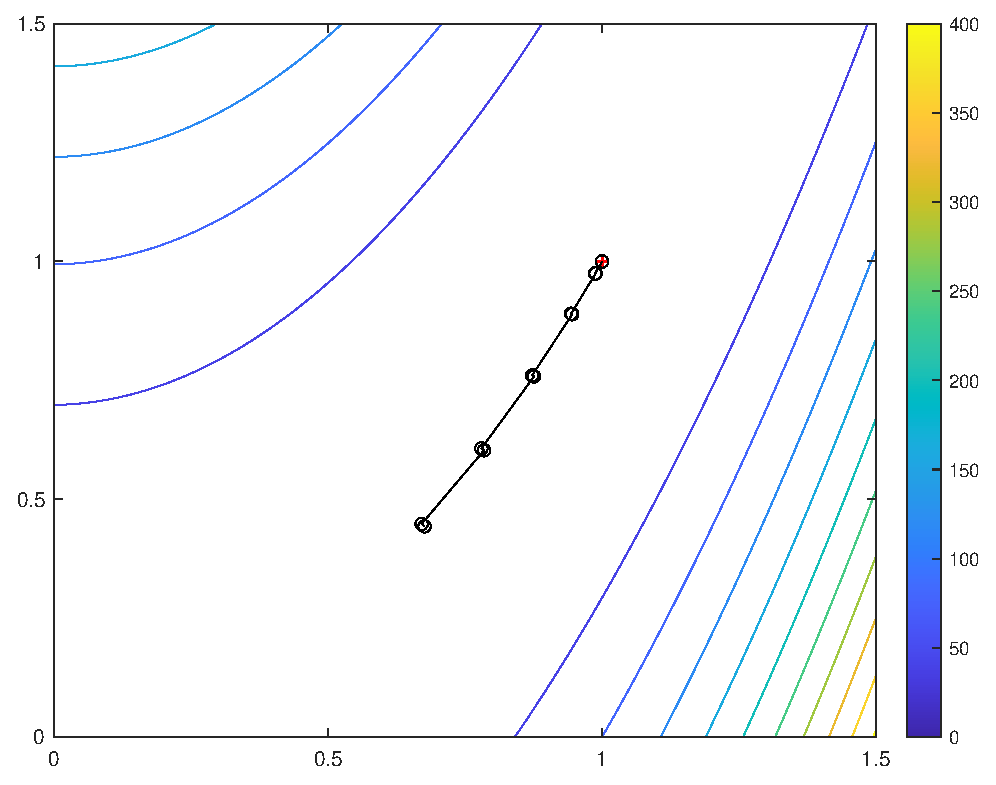
\includegraphics[width=11cm]{Image_6}
\caption{Conjugate Gradient Descent on Function (5)}\label{fg:Blah}
\end{figure}
We can see this method converges \textit{significantly} faster than in Question 3. This relaxed condition that iterates do not have to be perpendicular to one another means this method can travel along steep valleys in $f$ with far more ease. The iterates have separated into pairs, and this is explained when the method resets. This begs the question that this method may converge far faster if we do not reset it every $N$ steps. We will see below a proof that the conjugate gradient method always converges to $\x^{*}$ in both cases (resets and no resets) under certain assumptions.
\subsubsection*{\centering Convergence of Conjugate Gradient Method}
In order that $\lambda$ is well defined in each iterate, we assume that the level set $L=\lbrace \x : f(\x)\leq f(\x_{1})\rbrace \subset \R^{N}$ is bounded. We also assume that $f$ is twice continuously differentiable. We aim to show
\begin{equation}\label{eq:ConvConc}
\lim_{n\rightarrow \infty}\left(\inf_{k=0}^{n}\nabla f(\x_{k})\right)=0
\end{equation}
Since all iterates will remain in $L$, we can find an $M$ such that $f(\x)\preceq MI$, and thus
\begin{equation}
\begin{aligned}
f(\x_{n+1}) &\leq f(\x_{n})+(\x_{n+1}-\x_{n})^{T}\nabla f(\x_{n})+\frac{M}{2}\abs{\abs{\x_{n+1}-\x_{n}}}^{2}\\
&= f(\x_{n})+\lambda \s_{n}^{T}\nabla f(\x_{n})+\frac{M}{2}\lambda^{2}\abs{\abs{\s_{n}}}^{2}
\end{aligned}
\end{equation}
Notice this is true for all $\lambda$, so we may minimise the RHS by picking $\lambda=-\s_{n}^{T}\nabla f(\x_{n})/(M\abs{\abs{\s_{n}}}^{2})$, giving the new lower bound 
\begin{equation}
f(\x_{n+1}) \leq f(\x_{n})-\frac{1}{2M}\rho_{n}^{2}\abs{\abs{\nabla f(\x_{n})}}^{2}\\
\end{equation}
where \begin{equation}
\rho_{n}=\frac{\s_{n}^{T}\nabla f(\x_{n})}{\abs{\abs{\s_{n}}}\cdot \abs{\abs{\nabla f(\x_{n})}}}
\end{equation}
Since we assume that $f$ is bounded below, we deduce that 
\begin{equation}\label{eq:sumConv}
2M\left(f(\x_{1})-f(\x_{2})+f(\x_{2})-f(\x_{3})+\hdots\right) \geq \sum_{n=1}^{\infty}\rho_{n}^{2}\abs{\abs{\nabla f(\x_{n})}}^{2}
\end{equation}
must converge to some constant.\footnote{This gives a stronger proof of the convergence of the steepest descent algorithm in Question 3. In this case $\rho_{n}=-1$, and so we immediately deduce equation \eqref{eq:ConvConc}. Note we cannot deduce anything about the rate of convergence, unlike the proof given earlier.}\\

We now investigate how $\abs{\abs{\s_{n}}}$ behaves. We first claim that $\s_{i}^{T}\nabla f(\x_{i+1})=0$ for all $i$. This follows from a simple expansion of $d\phi /d\lambda =0$ at $\lambda^{*}$ where $\phi(\lambda)=f(\x_{i}+\lambda \s_{i})$. From this we can conclude that
\begin{equation}
\begin{aligned}
\abs{\abs{\s_{n}}}^{2} &=\abs{\abs{\nabla f(\x_{n})}}^{2}+\beta_{n}\abs{\abs{\s_{n-1}}}^{2}\\
&= \abs{\abs{\nabla f(\x_{n})}}^{2}+\beta_{n}^{2}\left(\abs{\abs{f(\x_{n-1})}}^{2}+\beta_{n-1}^{2}\abs{\abs{\s_{n-2}}}^{2}\right)=\hdots\\
&=\sum_{l=1}^{n}\prod_{j=l+1}^{n}\beta_{j}^{2}\abs{\abs{\nabla f(\x_{l})}}^{2}=\sum_{l=1}^{n}\frac{\abs{\abs{\nabla f(\x_{n})}}^{4}}{\abs{\abs{\nabla f(\x_{l})}}^{2}}
\end{aligned}
\end{equation}
where $\beta_{n}=\abs{\abs{\nabla f(\x_{n})}}^{2}/\abs{\abs{\nabla f(\x_{n-1})}}^{2}$ and the product in the last line is defined to be one if $l=n$. Suppose for contradiction that the gradients were bounded away from zero, and so the method did not converge. Then, since the iterates are assumed to remain in $L$, the gradients are bounded and so $\abs{\abs{\s_{n}}}^{2}\leq Cn$ for some positive constant $C$ (notice the same result is true if we allow the method to reset every $N$ steps), and thus the sum
\begin{equation}
\begin{aligned}
\sum_{n=1}^{\infty}\rho_{n}^{2} &=\sum_{n=1}^{\infty}\frac{\left(\left(-\nabla f(\x_{n})^{T}+\beta_{n-1}\s_{n-1}^{T}\right)\nabla f(\x_{n})\right)^{2}}{\abs{\abs{\s_{n}}}^{2}\cdot \abs{\abs{\nabla f(\x_{n})}}^{2}}\\
&=\sum_{n=1}^{\infty}\frac{\abs{\abs{\nabla f(\x_{n})}}^{2}}{\abs{\abs{\s_{n}}}^{2}}\\
&\geq\frac{\min_{n}\abs{\abs{\nabla f(\x_{n})}}^{2}}{C}\sum_{n=1}^{\infty}\frac{1}{n}
\end{aligned}
\end{equation}
diverges. However \eqref{eq:sumConv} always converges, and hence \eqref{eq:ConvConc} must be true, a contradiction. Hence the gradients cannot be bounded away from zero, and the conjugate gradient method always converges no matter the value of $\x_{0}$.\footnote{This proof was presented in \cite{GlobalConvergence}.}\\

The error $E_{n}=f(\x_{n})-f(\x^{*})$ was calculated every $N$ steps, just before the method would reset, and was plotted against $E_{n-N}$ on a log-log scale in Figure \ref{fg:0} below. 
\begin{figure}[H]
\centering
\includegraphics[width=10cm]{Regression_Line}
\caption{$\log (E_{(k+1)N})$ against $\log(E_{kN})$}\label{fg:0}
\end{figure}
 The least squares regression line was also calculated, however the last two points were omitted, sine they did not fit the trend. This is due to MATLAB not having the accuracy to store values to a high enough precision, and hence as we converge to the minimum $\x^{*}$, the method breaks down and the order of convergence will change. Initially, however, it's seen that $\log(E_{(k+1)N})$ decreases linearly against $\log(E_{kN})$ with estimated gradient $S_{XY}/S_{XX}=1.98$ (coefficient of determination $R^{2}=0.98$). Suppose that $\log(E_{(k+1)N})=m\log(E_{kN})+b$. Then $E_{(k+1)N}/(E_{kN})^{m}=C$ and the method is $m$-th order convergent every $N$ steps. 
 
 This agrees with our predictions in Question 4 that this method is close to 2nd order, and confirms that this is a far greater improvement over the steepest descent, especially when $N$ is small. It also makes intuitive sense this method will be faster than linear convergence, since if we assume the function $f$ behaves like a quadratic near it's minimum, then this method will almost exactly converge. At this point the function will behave even more so like a quadratic, and so we expect it to converge even better, and so forth. We therefore conjecture that all descent methods that converge exactly for quadratic functions will be faster than linear convergence. \\

To investigate the importance of the accuracy of $\lambda^{*}$, the method was run for different values of $d$ in the subroutine \texttt{lambda(x,s,d)}, and number of iterations required for the code to terminate is tabulated below in Table \ref{tb:10}. The termination criterion $\abs{\abs{\nabla f(\x_{i})}}\leq 10^{-7}$ was kept the same.
\begin{table}[H]
\centering
\begin{tabular}{|c|c|}
\hline $d$ & Num of iterates \\ \hline
2 & 88\\
3 & 49\\
4 & 15 \\
5 & 15\\
6 & 13\\
7 & 13\\
8 & 13 \\ \hline
\end{tabular}
\caption{Number of iterates for CGM with different $d$}\label{tb:10}
\end{table}
Firstly this is far more encouraging than the data in Table \ref{tb:2}, since as we increase the accuracy of $\lambda^{*}$, the number of iterations required to reach $\x^{*}$ decreases. However we still conclude that it is not worth calculating $\lambda^{*}$ to a very large accuracy, since we see little improvement with a large computational cost. Therefore it is most efficient to choose the accuracy of $\lambda^{*}$ around 4 significant figures. \\

We have seen that the conjugate gradient method is far more efficient than the steepest descent method with its quicker convergence. On the whole it is efficient, however one draw back is that numerically computers would quickly struggle to operate on such precise numbers. Because of this, the method would only work up until some fixed accuracy; thereafter it would deteriorate and the convergence becomes slow (as seen in Question 4).

\subsection*{\centering Question 6}
All results in Questions 6-8 were produced by '\nameref{cd:3}', referenced on page \pageref{cd:3}, including approximating the minimum of function (6) with the given values of $\lambda^{*}$. These iterates are plotted below in Table \ref{tb:4}.
\begin{table}[H]
\centering
\begin{tabular}{|ccccc|}
\hline
$n$ & $x_{n}$ & $y_{n}$ & $z_{n}$ & $f(\x_{n})$\\
\hline
0 & 1.0 & 1.0 & 1.0 & 2.6\\ 1 & 0.29044 & 0.84232 & -0.1826 & 0.15595116992\\ 2 & 0.12009759606 & -0.019151575072 & -0.067979309368 & 0.0022997644626\\ 3 & 4.3176483025e-6 & -4.2437453844e-5 & 2.6561522136e-5 & 1.1878421017e-9\\
\hline
True Value & 0 & 0 & 0 & 0\\
\hline
\end{tabular}
\caption{Iterates for DFP Algorithm for function (6)}\label{tb:4}
\end{table}
We can see that these iterates converge \textit{very} quickly towards the minimum, with the small amount of error due to $\lambda^{*}$ not being the exact minimums of $\phi(\lambda)$. The matrix $\mathbf{H}$ was calculated as
\begin{equation}
\begin{pmatrix}
3.3333333164 & 1.8954499403\times 10^{-7} & -1.6666667875\\ 1.8954499398\times 10^{-7} & 2.4999978441 & 1.3694454109\times 10^{-6}\\ -1.6666667875 & 1.3694454108\times 10^{-6} & 1.3333324628
\end{pmatrix}
\end{equation}
which again is very close to the value of the inverse Hessian (given in the project booklet), with the same above reason for it not being exact.\\

Suppose with each iteration the 'exact-line search' has an error tolerance for $\lambda^{*}$ of $\varepsilon$. Suppose that $\X_{n}$ denotes these slightly erroneous iterates, and $\mathbf{N}_{n}$ denote the erroneous $\mathbf{H}_{n}$. We aim to investigate how $E_{N}=\X_{N}-\x_{N}$ behaves as a function of $\varepsilon$. 

The first two iterates of this sequence will be equal to $\X_{0}=\x_{0}$ and $\X_{1}=\x_{0}+\varepsilon \s_{0}$. By a simple induction we can see that $\X_{k}=\x_{k}+\varepsilon \y_{k}+O(\varepsilon^{2})$ and $\mathbf{N}_{k}=\mathbf{H}_{n}+\varepsilon \mathbf{J}_{n}+O(\varepsilon^{2})$, for some $\y_{k}$ and $\mathbf{J}_{k}$. Assuming that $\nabla f(\x)$ is continuous, then $\X_{N}$ is a continuous function in $\varepsilon$ with $\X_{N}=\x_{N}$ when $\varepsilon =0$. So if $\varepsilon$ is chosen to be sufficiently small, we can assume that $\X_{N}$ lies in in the bounded set $L$ (where $L$ is defined in Question 5). Therefore
\begin{equation}
\begin{aligned}
f\left(\X_{N}\right) &=f\left(\x_{N}\right)+\varepsilon \nabla f\left(\x_{N}\right)^{T}\y_{N}+\frac{\varepsilon^{2}}{2}\y_{N}^{T}\G\y_{N} +O\left(\varepsilon^{3}\right)\\
&\leq f\left(\x^{*}\right)+\frac{C\varepsilon^{2}}{2}+O\left(\varepsilon^{3}\right)
\end{aligned}
\end{equation}
for some constant $C$, since $\X_{N}$ is bounded above. Therefore we expect the error to decay quadratically with variations in $\lambda^{*}$.\\

Sure enough this is true. By varying $\varepsilon=10^{-n}$ away from the given values of $\lambda^{*}$ for $1\leq n\leq 6$, the error was recorded and plotted on a log-log axis in Figure \ref{fg:6}.
\begin{figure}[H]
\centering
\includegraphics[width=11cm]{Image_Error}
\caption{$E_{n}$ due to variations in $\lambda^{*}$}\label{fg:6}
\end{figure}
Since $\log(E_{n})=m\log(\varepsilon)+b$, this suggests that $E_{n}=A\varepsilon^{m}$. The gradient was estimated as $1.9975$, with coefficient of determination $R^{2}=0.9995$. This confirms the above argument. Notice that no larger $n$ could be used in the above plot, since at this point the error of the fixed $\lambda^{*}$ would dominate $E_{n}$. 
\subsection*{\centering Question 7}
The iterates below in Table \ref{tb:5} were produced by '\nameref{cd:3}', referenced on page \pageref{cd:3}, by applying it to function (4). The accuracy of $\lambda^{*}$ was set to 6 significant figures. 
\begin{table}[H]
\centering
\begin{tabular}{|cccccc|} \hline $i$ & $x_{i}$ & $y_{i}$ & $\lambda^{*}$ & $f(\x_{i})$ & $\nabla f(\x_{i})$\\ 
\hline
0 & -1.0 & -1.3 & 0.082899 & 1.0561 & 7.96926\\ 
1 & -0.85990069 & -0.654382588 & 1.55071 & -1.021192093775325 & 0.294816\\ 
2 & -0.4101515060880377 & -0.7346911332893252 & 0.163979 & -1.087760859335732 & 0.284889\\ 
3 & -0.4183631534047471 & -0.780679513778455 & 1.77779 & -1.094571383343364 & 0.0282642\\ 
4 & -0.370247388564234 & -0.7942864568269687 & 0.148277 & -1.095274097407723 & 4.18258e-3\\ 
5 & -0.3700785953560684 & -0.7936896879475634 & 1.78282 & -1.095275394025928 & 2.27695e-5\\ 
6 & -0.3700394729826621 & -0.7937005176832045 & 0.148359 & -1.095275394488075 & 5.76315e-8\\ 
7 & -0.3700394752446549 & -0.7937005259287198 & 1.73 & -1.095275394488075 & 1.13071e-10\\ 
8 & -0.3700394750586982 & -0.7937005259840695 & -0.011111 & -1.095275394488075 & 1.13227e-11\\ 
9 & -0.3700394750587658 & -0.7937005259841755 & -0.00111 & -1.095275394488075 & 1.21056e-11\\ 
10 & -0.3700394750587702 & -0.7937005259841764 & $\ast$ & -1.095275394488075 & 1.21191e-11\\ \hline
\end{tabular}
\caption{DFP Algorithm on Function (4)}\label{tb:5}
\end{table}
We can see that it converges marginally quicker than the conjugate gradient method, with the termination criterion $\abs{\abs{\nabla f(\x_{i})}}\leq 10^{-7}$ being achieved after 6 iterations. The same problem occurs after this point; that MATLAB does not store values to a high enough precision, and hence the method breaks down. We will naturally focus on these first 6 iterations throughout the rest of the question. 
(The plot of these iterates have been excluded since it is too similar to Figure \ref{fg:5}). \\

Firstly the final value of $\h$ was equal to 
\begin{equation}
\begin{pmatrix} 1.666653774084148 & -0.4200064784744674\\ -0.4200064784744674 & 0.2644529620027095 \end{pmatrix}\approx \begin{pmatrix} 1 & 2^{2/3} \\ 2^{2/3} & 5\times 2^{1/3}\end{pmatrix}^{-1}=\G^{-1}
\end{equation}
suggesting that $\h$ also converges to $\G$ in the non-quadratic case (this will be discussed in greater detail in Question 8). To extrapolate the minimum, we can follow a similar method to the one in Question 4, by looking at how $A_{k}=f(\x_{(k+1)N})-f(\x_{kN})$ and $B_{k}=\abs{\abs{\x_{(k+1)N}-\x_{kN}}}$ behaves. Their values are tabulated below in Table \ref{tb:11}.
\begin{table}[H]
\centering
\begin{tabular}{|c|ccc|ccc|} \hline $k$ & $A_{k}$ & $A_{k}/A_{k-1}$ & $A_{k}/\left(A_{k-1}\right)^{2}$ & $B_{k}$ & $B_{k}/B_{k-1}$ & $B_{k}/\left(B_{k-1}\right)^{2}$ \\ \hline 0 & -2.143861 & $\ast$ & $\ast$ & 0.8170039 & $\ast$ & $\ast$\\ 
1 & -7.513238e-3 & 3.504536e-3 & -1.634685e-3 & 0.07172127 & 0.08778572 & 0.1074484\\ 
2 & -1.297080e-6 & 1.726393e-4 & -0.02297802 & 6.217343e-4 & 8.668757e-3 & 0.1208673\\ 
3 & -2.464537e-16 & 1.900065e-10 & -1.464879e-4 & 8.556535e-9 & 1.376236e-5 & 0.02213544\\ \hline
\end{tabular}
\caption{Table of differences for DFP Algorithm}\label{tb:11}
\end{table}
Once again we can see that this method is faster than linear convergence since column 3 is decreasing (discussed further in Question 8), and since the 4th and 7th columns appears to be roughly constant/decreasing, it's fair to assume that $A_{k}\approx \mu (A_{k-1})^{2}$, and $B_{k}\approx \eta (B_{k-1})^{2}$. Taking $\mu=-0.023$ and $\eta=0.12$, we can extrapolate (like in Question 4) to give 
\begin{equation}
\begin{aligned}
f(\x^{*}) \approx f(\x_{6})+A_{3}+\mu (A_{3})^{2} &=-1.095275394488075\\
\abs{\abs{\x_{6}-\x^{*}}} \lesssim B_{3}+\eta (B_{3})^{2} &= 8.56\times 10^{-9}
\end{aligned}
\end{equation}
Since the magnitude of $\abs{A_{3}}\leq 10^{-15}$ and $\eta (B_{3})^{2}\leq 10^{-17}$, they will make no contribution due to MATLAB's rounding error (15 sig figs). Comparing these results to the conjugate gradient method, we see it is fractionally more efficient, but not by much.
\subsection*{\centering Question 8}
The same program was used to iterate to find the minimum of function (5). The accuracy of $\lambda^{*}$ was still set to 6 significant figures, and it took 13 iterations for the code to terminate due to the condition $\abs{\abs{\nabla f(\x_{i})}}\leq 10^{-7}$, the same number as the conjugate gradient method. The iterates are tabulated below in Table \ref{tb:8}, however the graphical plot of these iterates has been omitted due to it's similarity with Figure \ref{fg:Blah}. 
\begin{table}[H]
\centering
\begin{tabular}{|ccccc|} 
\hline $i$ & $x_{i}$ & $y_{i}$ & $f(\x_{i})$ & $\nabla f(\x_{i})$ \\ \hline 
0 & 0.676 & 0.443 & 0.1206022861 & 3.262270091\\ 
1 & 0.67068000284751139 & 0.44800838771122692 & 0.1087118056 & 0.3962655588\\ 
2 & 0.78471391734013118 & 0.60298495348675518 & 0.05943682803 & 3.453158763\\ 
3 & 0.77967478062669637 & 0.60669282046542439 & 0.04865839136 & 0.2383643879\\ 
4 & 0.87576488546115661 & 0.75812174290403767 & 0.02168939497 & 2.640561396\\ 
5 & 0.87233523995551199 & 0.76029804445782678 & 0.01633428087 & 0.1270988565\\ 
6 & 0.94549977936688734 & 0.88887294498722058 & 0.005048535265 & 1.648896023\\ 
7 & 0.94354315009310041 & 0.88998634954330147 & 0.003193980425 & 0.05289421941\\ 
8 & 0.98810303369923980 & 0.97448608579175788 & 4.187581694e-4 & 0.6385261777\\ 
9 & 0.98738444781745993 & 0.97486502310917922 & 1.594699257e-4 & 0.01140014364\\ 
10 & 0.99979937197609359 & 0.99946210142354597 & 1.534826197e-6 & 0.04853472141\\ 
11 & 0.99974529989886096 & 0.99948939331293896 & 6.500144939e-8 & 2.278586580e-4\\ 
12 & 1.0000000135947638 & 0.99999999016072327 & 1.098754065e-13 & 1.327215260e-5\\ 
13 & 0.99999999877890200 & 0.99999999755169466 & 1.494066305e-18 & 1.092184140e-9 \\ \hline
\end{tabular}
\caption{DFP Iterates for function (5)}\label{tb:8}
\end{table}
We can immediately deduce that this, like all previous methods, converges to the minimum. The DFP algorithm does possess the property of global convergence for any sufficently smooth, differentiable function, however this has only been proved in the case $N=2$.\footnote{The proof of this can be found in \cite{Powell2Var}, however it has been omitted due to it's length and complexity.} It is currently unknown if in higher dimensions this method converges for all functions, however this does not affect us with the examples given in this project. \\

In order to investigate the convergence of this method, the $N$-th step error $E_{k}=f(\x_{kN})-0$ is tabulated below in Table \ref{tb:7}, along with $H_{n}=\abs{\abs{\h_{kN}-\G^{-1}}}$.
\begin{table}[H]
\centering
\begin{tabular}{|c|ccc|ccc|} \hline $k$ & $E_{k}$ & $E_{k}/E_{k-1}$ & $E_{k}/(E_{k-1})^{2}$ & $H_{k}$ & $H_{k}/H_{k-1}$ & $H_{k}/(H_{k-1})^{2}$ \\ \hline 
0 & 0.1206023 & $\ast$ & $\ast$ & 1.505002 & $\ast$ & $\ast$ \\ 
1 & 0.05943686 & 0.4928336 & 4.086437 & 1.883802 & 1.251694 & 0.8316887\\ 
2 & 0.02168949 & 0.3649164 & 6.139564 & 1.577138 & 0.8372101 & 0.4444258\\ 
3 & 5.048702e-3 & 0.2327719 & 10.73201 & 1.137967 & 0.7215393 & 0.4574991\\ 
4 & 4.187866e-4 & 0.08294936 & 16.42984 & 0.5333924 & 0.4687239 & 0.4118959\\ 
5 & 1.534586e-6 & 3.664362e-3 & 8.749951 & 0.06564057 & 0.1230624 & 0.2307165\\ 
6 & 1.026783e-13 & 6.690946e-8 & 0.04360099 & 7.913552e-4 & 0.01205589 & 0.1836652\\ \hline \end{tabular}
\caption{Error in DFP algorithm using function (5)}\label{tb:7}
\end{table}
First notice that the third column is decreasing, suggesting this method is faster than linear convergence, agreeing with the conjecture at the end of Question 5. The second column is approximately constant/decreasing, suggesting that this method is close to second order. Following a similar method to that in Question 5, we can calculate the least squares regression line of $\log(E_{(k+1)N})$ against $\log(E_{kN})$ to deduce that this method is approximately a 2.4-order convergent method (coefficient of determination $R^{2}=0.98$).\footnote{The scatter plot of these points has been omitted since the method is identical to Question 5.} It is faster than the 1.98 order convergence of the conjugate gradient method, but fractionally.

The norm between the matrix $\h_{kN}$ and the inverse Hessian has also been recorded, which can be seen tending to zero rapidly. In fact, the order of convergence of this matrix is calculated as 2.3 (coefficient of determination $R^{2}=0.99$), strangely close to order of this method. It suggests there may be some connection between the convergence of these two quantities, similar to the relation between these same quantities in the Symmetric Rank One method, and other Quasi-Newton methods. The final value of $\h_{kN}=\h_{12}$ was calculated as 

\begin{equation}
\begin{pmatrix}
0.4999478 & 0.9997680\\
0.9997680 & 2.0055315\\
\end{pmatrix}
\approx
\begin{pmatrix}
0.5 & 1\\
1 & 2.00625\\
\end{pmatrix}=\G^{-1}
\end{equation}

The sensitivity of $\lambda^{*}$ was recorded in a similar way to Question 5, with the number of iterations required to terminate ($\nabla f(\x_{i})\leq 10^{-7}$) being recorded for different values of $d$. The results are tabulated below in Table \ref{tb:12}.
\begin{table}[H]
\centering
\begin{tabular}{|c|c|}
\hline $d$ & Num of iterates\\
\hline 2 & 15\\
3 & 14\\
4 & 13\\
5 & 13\\
6 & 13\\
\hline
\end{tabular}
\caption{Number of iterates for DFP with different $d$}\label{tb:12}
\end{table}
This differs largely from the data in Table \ref{tb:10} when the conjugate gradient method was being used, and that the DFP method is far less sensitive to inaccuracies in $\lambda^{*}$. This is a large improvement, since little computational power has to be wasted calculating the minimum of $\phi(\lambda)$.

This method is not efficient when $N$ is large. With each iteration of this algorithm, $\h_{n}$ must be updated, which has complexity $O(N^{2})$, as opposed to the $O(N)$ iterations in the earlier methods. It also poses a marginally faster method than the conjugate gradient method, but not by much, and due to the codes inability to store values extremely accurately, this quality is lost. Another downfall is that there are faster Quasi-Newton methods that can be used with faster convergence with little to no extra computational cost, such as the BFGS algorithm. 


\subsection*{\centering Question 9}
We will calcluate the complexities of the three methods in terms of the final accuracy $\epsilon$ and $N$, all the while supposing that it takes a fixed number of operations to find the minimum of $\phi(\lambda)$.
Firstly the steepest descent method has complexity $O(N)$ for each iteration. If we require the final accuracy of the method to be less than $\epsilon$, then we require the number of iterates $n$ to satisfy
\begin{equation}
n>\frac{1}{\ln(\mu)}\ln\left(\frac{\epsilon}{E_{0}}\right)
\end{equation}
where $E_{0}$ is the initial error and $\mu$ is the ratio of consecutive errors. Hence we deduce that the complexity of this algorithm scales like $O\left(-N\ln\epsilon\right)$. 

Secondly note that if a method is $N$-step $p$-th order convergent (i.e. $E_{kN}= \mu \left( E_{(k-1)N}\right)^{p}$) where $p\neq 1$, then in order for the final accuracy to be less than $\epsilon$,
\begin{equation}
kN>\frac{N}{\ln(p)}\ln\left(\frac{\ln(\mu \epsilon)}{\ln(\mu E_{0})}\right)
\end{equation}
Therefore we deduce that the conjugate gradient method has complexity $O\left(N^{2}\ln\ln(1/\epsilon)\right)$, since just like the steepest descent method each iterate requires $O(N)$ operations, and that it's a $p=2$ method. Finally, for the DFP algorithm, since we continuously update the values of $\h$, each iterate takes $O(N^{2})$ operations. Although in this case $p=2.4$, this makes no major contribution to the complexity of the algorithm, and so we deduce that the method takes $O\left(N^{3}\ln\ln(1/\epsilon)\right)$. For clarity these complexities are tabulated below in Table \ref{tb:13}

\begin{table}[H]
\centering
\begin{tabular}{c|c|c}
SDM & CGM & DFP\\
\hline
$O\left(-N\ln\epsilon\right)$ & $O\left(N^{2}\ln\ln\left(1/\epsilon\right)\right)$ & $O\left(N^{3}\ln\ln\left(1/\epsilon\right)\right)$\\
\end{tabular}
\caption{Complexities of algorithms}\label{tb:13}
\end{table}
Firstly we notice that the CGM and DFP algorithms scale far worse with $N$ than the SDM, and so will not perform well when $N$ is large.\footnote{This is consistent with the results proved earlier in this project, with global convergence not being confirmed for the DFP algorithm when $N\geq 3$.} However when $N$ is small, these methods become far more efficient than the SDM, as observed, especially when $\epsilon$ shrinks to zero. \\

The CGM method appears superior to the DFP algorithm, however the crucial difference between them is that $\lambda^{*}$ must be calculated to a higher precision. This will consequently cause the CGM to run noticeably slower. Since the subroutine \texttt{lambda} was not required for this project, the complexity of it has not been investigated. It's interesting to see that the difference in orders of convergence between these two methods ($p=2$ and $2.4$) does not (majorly) affect the results, which seems counter-intuitive.\\

In conclusion, the SDM performs best when $N$ is large, the CGM method performs best when $N$ is large, $\epsilon$ is very small and the computational cost of minimising $\phi(\lambda)$ is small, and the DFP algorithm performs best when $N$ is small, $\epsilon$ is very small but the cost of minimising $\phi(\lambda)$ is large. \\

It is, however, very important to note that these conclusions are drawn from the assumption that the code can operate on arbitrarily accurate values. This is not the case, and although these results may hold for small $\epsilon$, the methods will break down after a certain threshold, after which the outcomes of the algorithms become far harder to predict. \\




\pagebreak
\section*{\centering References}\label{References}
\printbibliography[heading=none]
\pagebreak
\section*{\centering Code}
\subsection*{\centering \texttt{lambda(x,s,d)} Subroutine}\label{cd:0}
\begin{verbatim}
function [Approx,L] = lambda(x,s,d)
    Inc=10000000;
    Dif=vpa(func(x+Inc*s)-func(x));
    while Dif>0
            Inc=Inc/10;
            Dif=vpa(func(x+Inc*s)-func(x));
    end
    Counter=1;
    Approx=x;
    L=0;
    while Counter<=d
        Inc=Inc/10;
        SubCounter=1;
        Dif=vpa(func(Approx+SubCounter*Inc*s)-func(Approx+(SubCounter-1)*Inc*s));
        while Dif<0
            SubCounter=SubCounter+1;
            Dif=vpa(func(Approx+SubCounter*Inc*s)-func(Approx+(SubCounter-1)*Inc*s));
        end
        L=L+(SubCounter-2)*Inc;
        Approx=vpa(Approx+(SubCounter-2)*Inc*s);
        Counter=Counter+1;
    end
end
\end{verbatim}
\pagebreak

\subsection*{\centering Contour Plot Code}\label{cd:0.5}
\begin{verbatim}
figure
x=linspace(-1.5,1.5,1000);
y=linspace(-1.5,1.5,1000);
[X,Y]=meshgrid(x,y);
Z=func(X,Y);
contour(X,Y,Z,-1:0.4:7)
colorbar
hold on
scatter(2^(-2/3)-1,-2^(-1/3),'+','Red','LineWidth',1)
legend('','Minimum')
print('Image','-depsc')

function answer = func(x,y)
answer=x+y+x.^2./4-y.^2+(y.^2-x./2).^2;
end

% function answer = func(x,y)
% answer=(1-x).^2+80*(y-x.^2).^2;
% end
\end{verbatim}
\pagebreak

\subsection*{\centering SDM Code}\label{cd:1}
\begin{verbatim}
digits(16)
Point=[-1;-1.3];
Min=[2^(-2/3)-1;-2^(-1/3)];
LambdaSigFig=5;
Iterates=10;

tic
Iterations=zeros(1,10);
Iterations(1,1)=0;
Iterations(1,2)=Point(1);
Iterations(1,3)=Point(2);
Iterations(1,5)=vpa(func(Point));
Iterations(1,6)=norm(gradient(Point));

Counter=1;
n=1;
while n<Iterates+1
s=-gradient(Point);
Counter=Counter+1;
Iterations=[Iterations;zeros(1,10)];
Iterations(n+1,1)=n;

% %Plot of $phi(lambda)$ with prompt
Inc=10000000;
Dif=vpa(func(Point+Inc*s)-func(Point));
while Dif>0
        Inc=Inc/10;
        Dif=vpa(func(Point+Inc*s)-func(Point));
end
XPhi=linspace(0,5*Inc);
YPhi=zeros(1,100);
SubCounter=1;
while SubCounter<=100
    YPhi(SubCounter)=func(Point+XPhi(SubCounter)*s);
    SubCounter=SubCounter+1;
end
figure
plot(XPhi,YPhi)
prompt=input(sprintf('Enter %d-th lambda value: ',n));
close

% prompt=[];
if isempty(prompt)==1
    [Point,Iterations(Counter-1,4)]=lambda(Point,s,LambdaSigFig);
else
    Point=vpa(Point+prompt*s);
    Iterations(Counter-1,4)=prompt;
end


Iterations(Counter,2)=Point(1);
Iterations(Counter,3)=Point(2);
Iterations(Counter,5)=vpa(func(Point));
Iterations(Counter,6)=norm(gradient(Point));
Iterations(Counter,7)=Iterations(Counter,5)-Iterations(Counter-1,5);
Iterations(Counter,8)=Iterations(Counter,7)/Iterations(Counter-1,7);
Iterations(Counter,9)=norm(Point-[Iterations(Counter-1,2);Iterations(Counter-1,3)]);
if Counter>=3
    Iterations(Counter,10)=Iterations(Counter,9)/Iterations(Counter-2,9);
end

%Termination Process
% if norm(s)<=10^-7
%     disp('Termination - Gradient small')
%     break
% end
% if (Iterations(n+1,2)-Iterations(n,2))^2+...
%         (Iterations(n+1,3)-Iterations(n,3))^2<=10^-20
%     disp('Termination - Iterations close together')
%     break
% end
n=n+1;
end
disp(Iterations)
latex(sym(vpa(Iterations)))

% disp(norm(Point-[1;1]))

figure
x=linspace(-1.5,0);
y=linspace(-1.5,0);
SupCounter=1;
Z=zeros(100,100);
while SupCounter<=100
    SubCounter=1;
    while SubCounter<=100
        Z(SubCounter,SupCounter)=func([x(SupCounter);y(SubCounter)]);
        SubCounter=SubCounter+1;
    end
    SupCounter=SupCounter+1;
end
contour(x,y,Z)
colorbar
hold on
scatter(Min(1),Min(2),'+','Red','LineWidth',1)
plot(Iterations(:,2),Iterations(:,3),'k')
scatter(Iterations(:,2),Iterations(:,3),'k')
print('Image','-depsc')

toc

%FUNCTIONS TO INTERCHANGE

function answer = func(x)
answer=x(1)+x(2)+x(1)^2/4-x(2)^2+(x(2)^2-x(1)/2)^2;
end

function answer = gradient(x)
answer=[1+x(1)-x(2)^2;1-4*x(2)*(-x(2)^2+x(1)/2)-2*x(2)];
end

% function answer = func(x)
% answer=(1-x(1))^2+80*(x(2)-x(1)^2)^2;
% end
% 
% function answer = gradient(x)
% answer=[320*x(1)^3+(2-320*x(2))*x(1)-2;160*(x(2)-x(1)^2)];
% end
\end{verbatim}
\pagebreak

\subsection*{\centering CGM Code}\label{cd:2}
\begin{verbatim}
digits(16)
NewPoint=[-1;-1.3];
Min=[2^(-2/3)-1,-2^(-1/3)];
N=2;
LambdaSigFig=5;

Iterates=10;

tic
Iterations=zeros(Iterates+1,N+4);
Iterations(1,1)=0;
Counter=1;
while Counter<=N
    Iterations(1,Counter+1)=NewPoint(Counter);
    Counter=Counter+1;
end

Iterations(1,N+3)=vpa(func(NewPoint));
Iterations(1,N+4)=norm(grad(NewPoint));

Differences=zeros(floor(Iterates/N),7);
Index=1;
LowerPoint=NewPoint;

n=0;
while n<Iterates
    if mod(n,N)==0
        s=-grad(NewPoint);
    else
        s=-grad(NewPoint)+norm(grad(NewPoint))^2/norm(grad(OldPoint))^2*s;
    end
    OldPoint=NewPoint;
    

%     %Plot of $phi(lambda)$ with prompt
    Inc=10000000;
    Dif=vpa(func(NewPoint+Inc*s)-func(NewPoint));
    while Dif>0
            Inc=Inc/10;
            Dif=vpa(func(NewPoint+Inc*s)-func(NewPoint));
    end
    XPhi=linspace(0,5*Inc);
    YPhi=zeros(1,100);
    SubCounter=1;
    while SubCounter<=100
        YPhi(SubCounter)=func(NewPoint+XPhi(SubCounter)*s);
        SubCounter=SubCounter+1;
    end
    figure
    plot(XPhi,YPhi)
    prompt=input(sprintf('Enter %d-th lambda value: ',n+1));
    close

%     prompt=[];
    if isempty(prompt)==1
        [NewPoint,Iterations(n+1,N+2)]=lambda(NewPoint,s,LambdaSigFig);
    else
        NewPoint=vpa(NewPoint+prompt*s);
        Iterations(n+1,N+2)=prompt;
    end

    Iterations(n+2,1)=n+1;
    Counter=1;
    while Counter<=N
        Iterations(n+2,Counter+1)=NewPoint(Counter);
        Counter=Counter+1;
    end
    Iterations(n+2,N+3)=vpa(func(NewPoint));
    Iterations(n+2,N+4)=vpa(norm(grad(NewPoint)));

    if and(mod(n+1,N)==0,n~=0)
        Differences(Index,1)=Index-1;
        Differences(Index,2)=vpa(func(NewPoint))-vpa(func(LowerPoint));
        Differences(Index,5)=norm(vpa(NewPoint)-vpa(LowerPoint));
        if Index~=1
            Differences(Index,3)=Differences(Index,2)/Differences(Index-1,2);
            Differences(Index,4)=Differences(Index,2)/Differences(Index-1,2)^2;
            Differences(Index,6)=Differences(Index,5)/Differences(Index-1,5);
            Differences(Index,7)=Differences(Index,5)/Differences(Index-1,5)^2;
        end
        LowerPoint=vpa(NewPoint);
        Index=Index+1;
    end

% TERMINATION PROCESS
%     if Iterations(n+2,N+4)<=10^-7
%         disp('Termination - Gradient small')
%         break
%     end
%     if norm(NewPoint-OldPoint)<=10^-10
%         disp('Termination - Iterations close together')
%         break
%     end
    n=n+1;
end
toc

disp(Iterations)
latex(sym(vpa(Iterations)))

% disp(Differences)
% latex(sym(vpa(Differences)))

% PLOT ITERATES
figure
x=linspace(-1.5,0);
y=linspace(-1.5,0);
SupCounter=1;
Z=zeros(100,100);
while SupCounter<=100
    SubCounter=1;
    while SubCounter<=100
        Z(SubCounter,SupCounter)=func([x(SupCounter);y(SubCounter)]);
        SubCounter=SubCounter+1;
    end
    SupCounter=SupCounter+1;
end
contour(x,y,Z)
colorbar
hold on
scatter(Min(1),Min(2),'+','Red','LineWidth',1)
plot(Iterations(:,2),Iterations(:,3),'k')
scatter(Iterations(:,2),Iterations(:,3),'k')
print('Image','-depsc')


%ERROR ANAYLISIS FOR FUNCTION (5)
% figure
% x=zeros(floor(Iterates/2),1);
% y=zeros(floor(Iterates/2),1);
% Counter=1;
% while Counter<=floor(Iterates/2)
%     x(Counter)=log(Iterations(2*Counter-1,N+3));
%     y(Counter)=log(Iterations(2*Counter+1,N+3));
%     Counter=Counter+1;
% end
% X=x(1:end-2);
% Y=y(1:end-2);
% m=(sum(X.*Y)-sum(X)*sum(Y)/(size(X,1)))/(sum(X.^2)-sum(X)^2/(size(X,1)));
% b=(sum(Y)-m*sum(X))/size(X,1);
% z=m*x+b;
% Z=m*X+b;
% plot(x,z)
% hold on
% scatter(x,y)
% xlabel('log E_{kN}')
% ylabel('log E_{(k+1)N}')
% legend('Least Squares Regression Line','','Location','northwest')
% print('Regression Line','-depsc')
% R=1-sum((Y-Z).^2)/(sum((Y-(sum(Y)/size(Y,1))).^2));

%FUNCTIONS TO INTERCHANGE

function answer = func(x)
answer=vpa(x(1)+x(2)+x(1)^2/4-x(2)^2+(x(2)^2-x(1)/2)^2);
end

function answer = grad(x)
answer=vpa([1+x(1)-x(2)^2;1-4.*x(2)*(-x(2)^2+x(1)/2)-2.*x(2)]);
end

% function answer = func(x)
% answer=(1-x(1))^2+80*(x(2)-x(1)^2)^2;
% end
% 
% function answer = grad(x)
% answer=[320*x(1)^3+(2-320*x(2))*x(1)-2;160*(x(2)-x(1)^2)];
% end
\end{verbatim}
\pagebreak

\subsection*{\centering DFP Code}\label{cd:3}
\begin{verbatim}
digits(16)
NewPoint=[1;1;1];
Min=[0,0,0];
N=3;
LambdaSigFig=5;
Iterates=3;

[Iterations,Differences,Errors]=DFP_Algorithm(NewPoint,N,LambdaSigFig,Iterates);
disp(Iterations)
% disp(Differences)
% disp(Errors)
latex(sym(vpa(Iterations)))
% latex(sym(vpa(Differences)))
% latex(sym(vpa(Errors)))

% QUESTION 7-8
% figure
% x=linspace(0,1.5);
% y=linspace(0,1.5);
% SupCounter=1;
% Z=zeros(100,100);
% while SupCounter<=100
%     SubCounter=1;
%     while SubCounter<=100
%         Z(SubCounter,SupCounter)=func([x(SupCounter);y(SubCounter)]);
%         SubCounter=SubCounter+1;
%     end
%     SupCounter=SupCounter+1;
% end
% contour(x,y,Z)
% colorbar
% hold on
% scatter(Min(1),Min(2),'+','Red','LineWidth',1)
% plot(Iterations(:,2),Iterations(:,3),'k')
% scatter(Iterations(:,2),Iterations(:,3),'k')
% print('Image','-depsc')

% QUESTION 8
% figure
% X=log(Errors(1:6,5));
% Y=log(Errors(2:7,5));
% scatter(X,Y)
% hold on
% m=(sum(X.*Y)-sum(X)*sum(Y)/(size(X,1)))/(sum(X.^2)-sum(X)^2/(size(X,1)));
% b=(sum(Y)-m*sum(X))/size(X,1);
% Z=m*X+b;
% R=1-sum((Y-Z).^2)/(sum((Y-(sum(Y)/size(Y,1))).^2));
% plot(X,Z)

% QUESTION 6
Counter=1;
X=zeros(1,6);
Y=zeros(1,6);
while Counter<=6
    X(Counter)=log(10^(-Counter));
    Table=DFP_Algorithm(NewPoint,N,LambdaSigFig,Iterates);
    Y(Counter)=log(Table(end,N+3));
    Counter=Counter+1;
end
figure
m=(sum(X.*Y)-sum(X)*sum(Y)/(size(X,2)))/(sum(X.^2)-sum(X)^2/(size(X,2)));
b=(sum(Y)-m*sum(X))/size(X,2);
r=1-sum((Y-(b+m*X)).^2)/sum((Y-sum(Y)/6).^2);
Z=m*X+b;
plot(X,Z);
hold on
scatter(X,Y)
xlabel('log \epsilon')
ylabel('log E_{n}')
legend('Least Squares Regression Line','Location','northwest')
print('Image_Error','-depsc')


function [Iterations,Differences,Error] = DFP_Algorithm(NewPoint,N,LambdaSigFig,Iterates)
tic
Iterations=zeros(1,N+4);
Iterations(1,1)=0;
Counter=1;
while Counter<=N
    Iterations(1,Counter+1)=NewPoint(Counter);
    Counter=Counter+1;
end
Iterations(1,N+3)=func(NewPoint);
Iterations(1,N+4)=norm(grad(NewPoint));


Differences=zeros(floor(Iterates/N),7);
Index=1;
LowerPoint=NewPoint;

%QUESTION 8
% G=[1/2 1;1 321/160];
Error=zeros(floor(Iterates/N),7);
% Error(Index,1)=0;
% Error(Index,2)=vpa(func(NewPoint));
% Error(Index,5)=norm(eye(N)-G);

n=0;
while n<Iterates
    if mod(n,N)==0
        H=eye(N);
    end
    s=-H*grad(NewPoint);
    OldPoint=NewPoint;

    %Plot of $phi(lambda)$ with prompt
    Inc=10000000;
    Dif=vpa(func(NewPoint+Inc*s)-func(NewPoint));
    while Dif>0
            Inc=Inc/10;
            Dif=vpa(func(NewPoint+Inc*s)-func(NewPoint));
    end
    XPhi=linspace(0,5*Inc);
    YPhi=zeros(1,100);
    SubCounter=1;
    while SubCounter<=100
        YPhi(SubCounter)=func(NewPoint+XPhi(SubCounter)*s);
        SubCounter=SubCounter+1;
    end
    figure
    plot(XPhi,YPhi)
    prompt=input(sprintf('Enter %d-th lambda value: ',n+1));
    close

%     prompt=[];
    if isempty(prompt)==1
        [NewPoint,Iterations(n+1,N+2)]=lambda(NewPoint,s,LambdaSigFig);
    else
        NewPoint=vpa(NewPoint+prompt*s);
        Iterations(n+1,N+2)=prompt;
    end

    Iterations(n+2,1)=n+1;
    Counter=1;
    while Counter<=N
        Iterations(n+2,Counter+1)=NewPoint(Counter);
        Counter=Counter+1;
    end
    Iterations(n+2,N+3)=vpa(func(NewPoint));
    Iterations(n+2,N+4)=norm(grad(NewPoint));
    p=grad(NewPoint)-grad(OldPoint);
    q=NewPoint-OldPoint;
    H=H-H*(p*p')*H/(p'*H*p)+q*q'/(p'*q);

    if and(mod(n+1,N)==0,n~=0)
        Differences(Index,1)=Index-1;
        Differences(Index,2)=vpa(func(NewPoint))-vpa(func(LowerPoint));
        Differences(Index,5)=norm(vpa(NewPoint)-vpa(LowerPoint));
        if Index~=1
            Differences(Index,3)=Differences(Index,2)/Differences(Index-1,2);
            Differences(Index,4)=Differences(Index,2)/Differences(Index-1,2)^2;
            Differences(Index,6)=Differences(Index,5)/Differences(Index-1,5);
            Differences(Index,7)=Differences(Index,5)/Differences(Index-1,5)^2;
        end
        LowerPoint=vpa(NewPoint);
        
%         QUESTION 8
%         Error(Index+1,1)=Index;
%         Error(Index+1,2)=vpa(func(NewPoint));
%         Error(Index+1,3)=Error(Index+1,2)/Error(Index,2);
%         Error(Index+1,4)=Error(Index+1,2)/(Error(Index,2)^2);
%         Error(Index+1,5)=norm(H-G);
%         Error(Index+1,6)=Error(Index+1,5)/Error(Index,5);
%         Error(Index+1,7)=Error(Index+1,5)/(Error(Index,5)^2);
        Index=Index+1;
    end

% % TERMINATION PROCESS
    if Iterations(n+2,N+4)<=10^-7
        disp('Termination - Gradient small')
        break
    end
    if norm(NewPoint-OldPoint)<=10^-10
        disp('Termination - Iterations close together')
        break
    end
    disp(H)
    n=n+1;
end
toc
end

%FUNCTIONS TO INTERCHANGE

% function answer = func(x)
% answer=x(1)+x(2)+x(1)^2/4-x(2)^2+(x(2)^2-x(1)/2)^2;
% end
% 
% function answer = grad(x)
% answer=[1+x(1)-x(2)^2;1-4.*x(2)*(-x(2)^2+x(1)/2)-2.*x(2)];
% end

% function answer = func(x)
% answer=(1-x(1))^2+80*(x(2)-x(1)^2)^2;
% end
% 
% function answer = grad(x)
% answer=[320*x(1)^3+(2-320*x(2))*x(1)-2;160*(x(2)-x(1)^2)];
% end

function answer = func(x)
    answer = 0.4*x(1)^2+0.2*x(2)^2+x(3)^2+x(1)*x(3);
end

function answer = grad(x)
    answer = [0.8*x(1)+x(3);0.4*x(2);2*x(3)+x(1)];
end
\end{verbatim}
\pagebreak


\end{document}
